
\chapter{Free Strict $n$-Categories}
\lbl{app:free-strict}%
%
\index{n-category@$n$-category!strict!free|(}%
%
\index{omega-category@$\omega$-category!strict!free|(}
%


\noindent
Here we prove that the forgetful functor
\[
(\textrm{strict } n \textrm{-categories} )
\go
(n\textrm{-globular sets})
\]
is monadic and that the induced monad is cartesian and finitary.  We also
prove the analogous results for $\omega$-categories.  We used monadicity
and that the monad is cartesian in Part~\ref{part:n-categories}, in order
to be able to define and understand globular operads and weak $n$- and
$\omega$-categories.  We use the fact that the monad is finitary for
technical purposes in Appendix~\ref{app:initial}.

It is frustrating to have to prove this theorem, for two separate reasons.
The first is that the proof can \emph{almost} be made trivial: an adjoint
functor theorem tells us that the forgetful functor has a left adjoint, a
monadicity theorem tells us that it is monadic, and a routine calculation
tells us that it is finitary.  However, we have no result of the form
`given an adjunction, its induced monad is cartesian if the right adjoint
satisfies certain conditions', and so in order to prove that the monad is
cartesian we are forced to actually construct the whole adjunction
explicitly.  The second is that there ought to be some way of simply
looking at the theory of strict $\omega$-categories, presented as an
algebraic theory on the presheaf category of globular sets (as
in~\ref{defn:strict-n-cat-glob}), and applying some general principle to
deduce the theorem immediately; see p.~\pageref{p:sr-presheaf}.  But
again, we currently have no way of doing this.

Despite these frustrations, the proof is quite easy.  By exploiting the
definition of strict $n$- and $\omega$-categories by iterated
enrichment~(\ref{defn:strict-n-cat-enr}), we can reduce it to the proof of
some straightforward statements about enriched categories.

Here is the idea.  Suppose we know how to construct the free strict
2-category on a 2-globular set.  Then we can construct the free strict
3-category on a 3-globular set $X$ in two steps:
%
\begin{itemize}
  \item For each $x, x' \in X(0)$, take the 2-globular set $X(x,x')$ of
  cells whose 0-dimensional source is $x$ and whose 0-dimensional target is
  $x'$, replace it by the free strict 2-category on $X(x,x')$, and
  reassemble to obtain a new 3-globular set $Y$.  The $0$- and $1$-cells of
  $Y$ are the same as those of $X$, and a typical 3-cell of $Y$ looks
  like
  \[
\setlength{\unitlength}{1mm}
\begin{picture}(70,56)(-35,-28)
\cell{0}{0.5}{c}{\includegraphics{3pd.eps}}
\cell{-32}{0}{r}{x}
\cell{32}{0}{l}{x'}
\cell{15}{26}{c}{\scriptstyle f_0}
\cell{15}{9}{c}{\scriptstyle f_1}
\cell{15}{-9}{c}{\scriptstyle f_2}
\cell{15}{-25}{c}{\scriptstyle f_3}
\cell{-14}{17}{c}{\scriptstyle \alpha_0}
\cell{2}{15}{c}{\scriptstyle \alpha_1}
\cell{14}{17}{c}{\scriptstyle \alpha_2}
\cell{-9}{0}{c}{\scriptstyle \beta_0}
\cell{9}{0}{c}{\scriptstyle \beta_1}
\cell{-14}{-18}{c}{\scriptstyle \gamma_0}
\cell{2}{-20}{c}{\scriptstyle \gamma_1}
\cell{14}{-18}{c}{\scriptstyle \gamma_2}
\cell{-6}{19}{b}{\scriptstyle \Gamma_1}
\cell{6}{19}{b}{\scriptstyle \Gamma_2}
\cell{0}{1}{b}{\scriptstyle \Delta_1}
\cell{-6}{-17}{b}{\scriptstyle \Theta_1}
\cell{6}{-17}{b}{\scriptstyle \Theta_2}
\end{picture}
%   \hand{70}{48}
  \]
  where $x$ and $x'$ are 0-cells of $X$, the $f_i$'s are 1-cells, the
  $\alpha_i$'s, $\beta_i$'s and $\gamma_i$'s are 2-cells, and the
  $\Gamma_i$'s, $\Delta_i$'s and $\Theta_i$'s are 3-cells.
  
  \item Write $\cat{A}$ for the category of 2-globular sets, think of $Y$
  as a family $(Y(x,x'))_{x, x'\in X(0)}$ of objects of $\cat{A}$, and let
  $Z$ be the free $\cat{A}$-enriched category on $Y$.  The $0$-cells of $Z$
  are the same as those of $X$ and $Y$, and a typical 3-cell of $Z$ looks
  like
  \[
  \includegraphics{long3pd.eps}
%   \hand{45}{49}
  \]
  where the cells making up this diagram are cells of $X$.  So $Z$ is the
  free strict 3-category on $X$.
\end{itemize}
%
We therefore construct the free strict $n$-category functor inductively on
$n$, and pass to the limit to reach the infinite-dimensional version. 

In the first section,~\ref{sec:free-enr}, we prove the necessary results on
free enriched categories.  In the second,~\ref{sec:free-n}, we apply them
to establish the existence and properties of the free strict $n$- and
$\omega$-category functors.  Since the construction is explicit, we are
then able to verify the intuitively plausible formula~\bref{eq:pd-rep-of-T}
(p.~\pageref{eq:pd-rep-of-T}) for the free functor in terms of pasting
diagrams.


\section{Free enriched categories}
\lbl{sec:free-enr}%
%
\index{category!free enriched|(}%
%
\index{enrichment!category@of category!finite product category@in finite product category|(}
%

Recall from~\ref{sec:cl-enr} that for every category $\cat{A}$ there is a
category $\cat{A}\hyph\Gph$ of $\cat{A}$-graphs, and that if $\cat{A}$ has
finite products then there is also a category $\cat{A}\hyph\Cat$ of
$\cat{A}$-enriched categories and a forgetful functor $\cat{A}\hyph\Cat \go
\cat{A}\hyph\Gph$.  Any finite-product-preserving functor $Q: \cat{B} \go
\cat{A}$ between categories with finite products induces a (strictly)
commutative square
%
\[
\begin{diagram}[size=2em]
\cat{B}\hyph\Cat	&\rTo	&\cat{A}\hyph\Cat	\\
\dTo			&	&\dTo			\\
\cat{B}\hyph\Gph	&\rTo	&\cat{A}\hyph\Gph,	\\
\end{diagram}
\]
and in particular induces an unambiguous functor $\cat{B}\hyph\Cat \go
\cat{A}\hyph\Gph$.  So if $T$ is a monad on a category $\cat{A}$ with
finite products then the forgetful functor $\cat{A}^T \go \cat{A}$ induces
a forgetful functor $\cat{A}^T\hyph\Cat \go \cat{A}\hyph\Gph$.  This
functor will play an important role.

A monad will be called \demph{coproduct-preserving}%
%
\index{coproduct!preserved by monad}%
%
\index{monad!coproduct-preserving}
%
%
if its functor part
preserves all (small) coproducts.

\begin{propn}	\lbl{propn:free-enr}
Let $\cat{A}$ be a presheaf category.
%
\begin{enumerate}
\item	\lbl{item:free-enr-simple}
The forgetful functor 
\[
\cat{A}\hyph\Cat \go \cat{A}\hyph\Gph
\]
is monadic, and the induced monad is cartesian, finitary and
coproduct-preserving.
\item	\lbl{item:free-enr-graphs}
For any monad $T$ on $\cat{A}$, the forgetful functor 
\[
\cat{A}^T\hyph\Gph \go \cat{A}\hyph\Gph
\]
is monadic, and the induced monad is cartesian (respectively, finitary or
coproduct-preserving) if $T$ is.
\item	\lbl{item:free-enr-both}
For any coproduct-preserving monad $T$ on $\cat{A}$, the forgetful functor 
\[
\cat{A}^T\hyph\Cat \go \cat{A}\hyph\Gph
\]
is monadic; the induced monad $\newmnd{T}$ is coproduct-preserving, and is
cartesian (respectively, finitary) if $T$ is.
\end{enumerate}
%
Moreover, $\newmnd{T}$ 
is given on $\cat{A}$-graphs $X$ by $(\newmnd{T}X)_0 = X_0$ and
\[
(\newmnd{T}X)(x,x') 
=
\coprod_{x=x_0, x_1, \ldots, x_{r-1}, x_r=x'}
T(X(x_0, x_1)) \times\cdots\times T(X(x_{r-1},x_r))
\]
($x,x' \in X_0$), where the coproduct is over all $r\in\nat$ and sequences
$x_0, \ldots, x_r$ of elements of $X_0$ satisfying $x_0 = x$ and $x_r =
x'$.
\end{propn}
%
The hypothesis that $\cat{A}$ is a presheaf category is excessive, but
makes the proof easier and serves our purpose.
%
\begin{proof}
Part~\bref{item:free-enr-simple} is simple: free $\cat{A}$-enriched
categories are constructed just as free ordinary categories are.
The induced monad $\fc_\cat{A}$ on $\cat{A}\hyph\Gph$ is given on
$\cat{A}$-graphs $X$ by $(\fc_\cat{A} X)_0 = X_0$ and
\[
(\fc_\cat{A}X)(x,x')
=
\coprod_{x=x_0, x_1, \ldots, x_{r-1}, x_r=x'}
X(x_0, x_1) \times\cdots\times X(x_{r-1},x_r)
\]
($x,x' \in X_0$).  Everything works as in the familiar case $\cat{A}=\Set$
because $\cat{A}$ is a $\Set$-valued functor category.

Part~\bref{item:free-enr-graphs} is also straightforward: $\blank\hyph\Gph$
defines a strict map $\CAT \go \CAT$ of strict 2-categories (ignoring
set-theoretic worries), and so turns the adjunction between $\cat{A}^T$ and
$\cat{A}$ into an adjunction between the corresponding categories of
graphs.  Explicitly, the induced monad $T_*$ on $\cat{A}\hyph\Gph$ is given
on $\cat{A}$-graphs $X$ by $(T_* X)_0 = X_0$ and $(T_* X)(x,x') =
T(X(x,x'))$.  That $T_*$ inherits the properties of $T$ is easily checked.

To prove~\bref{item:free-enr-both} and `moreover' it suffices to put a
monad structure on the composite functor $\fc_\cat{A} \of T_*$, to
construct an isomorphism of categories
\[
(\cat{A}\hyph\Gph)^{\fc_\cat{A} \of T_*} \iso \cat{A}^T\hyph\Cat
\]
commuting with the forgetful functors to $\cat{A}\hyph\Gph$, and to check
that the monad $\fc_\cat{A} \of T_*$ is cartesian if $T$ is.  (Recall the
two-step strategy of the introduction.)  The monad structure on
$\fc_\cat{A} \of T_*$ consists of the monad structures on $T_*$ and
$\fc_\cat{A}$ glued together by a distributive%
%
\index{distributive law}
%
law~(\ref{defn:distrib-law})
\[
\lambda: T_* \of \fc_\cat{A} \go \fc_\cat{A} \of T_*.
\]
The functor $\fc_\cat{A} \of T_*$ is given by the formulas for $\newmnd{T}$
in `moreover'; the composite the other way round is given by $((T_* \of
\fc_\cat{A})(X))_0 = X_0$ and
\[
((T_* \of \fc_\cat{A})X)(x,x') 
=
\coprod_{x=x_0, x_1, \ldots, x_{r-1}, x_r=x'}
T(X(x_0, x_1) \times\cdots\times X(x_{r-1},x_r)).
\]
So we can define $\lambda_X$ by the evident natural maps.  It is
straightforward to check that $\lambda$ is indeed a distributive law and
that $\lambda$ is cartesian if $T$ is, so the monad $\fc_\cat{A} \of T_*$
is cartesian if $T$ is~(\ref{lemma:distrib-gives-monad}).  All that remains
is the isomorphism.  That follows from~\ref{lemma:distrib-iso-algs} once we
know that the monad on $(\cat{A}\hyph\Gph)^{T_*} \iso \cat{A}^T\hyph\Gph$
corresponding to the distributive law $\lambda$ is $\fc_{\cat{A}^T}$, and
that too is easily checked.  \done
\end{proof}%
%
\index{category!free enriched|)}%
%
\index{enrichment!category@of category!finite product category@in finite product category|)}
%





\section{Free $n$- and $\omega$-categories}
\lbl{sec:free-n}%
%
\index{enrichment!define n-category@to define $n$-category|(}
%

Since we are using the definition of strict $n$- and $\omega$-categories by
iterated enrichment, it is convenient to replace the category of
$n$-globular sets by the equivalent category $n\hyph\Gph$ of $n$-graphs%
%
\index{n-graph@$n$-graph|(}
%
introduced in~\ref{propn:str-n-cats-comparison}.  There is a forgetful
functor $U_n: \strc{n} \go n\hyph\Gph$ defined by taking $U_0$ to be the
identity and $U_{n+1}$ to be the diagonal of the commutative square
%
\begin{equation}	\label{diag:cat-gph-square}
\begin{diagram}[size=2em]
(\strc{n})\hyph\Cat	&\rTo	&(n\hyph\Gph)\hyph\Cat	\\
\dTo			&	&\dTo			\\
(\strc{n})\hyph\Gph	&\rTo	&(n\hyph\Gph)\hyph\Gph.	\\
\end{diagram}
\end{equation}
%
(We abbreviate our previous notation for the category of strict
$n$-categories, \strcat{n}, to \strc{n}.)  There is also a restriction
functor $R_n: (n+1)\hyph\Gph \go n\hyph\Gph$%
% 
\glo{Rngraphs}
% 
for each $n\in\nat$, defined
by $R_0(X) = X_0$ and $R_{n+1} = R_n\hyph\Gph$.  These functors fit
together into a strictly commutative diagram
\[
\begin{diagram}[height=2em,width=3em] %[size=3em,tight]
\cdots		&\strc{(n+1)}	&\rTo^{S_n}	
&\strc{n}	&\rTo^{S_{n-1}}	&\ &\cdots&\ &\rTo^{S_0}&\strc{0}	\\
		&\dTo>{U_{n+1}}	&		
&\dTo>{U_n}	&		&&	&&		&\dTo>{U_0}	\\
\cdots		&(n+1)\hyph\Gph	&\rTo_{R_n}	
&n\hyph\Gph	&\rTo_{R_{n-1}}	&\ &\cdots&\ &\rTo_{R_0}&0\hyph\Gph,	\\
\end{diagram}
\]
where the functors $S_n$ are the usual ones
(p.~\pageref{p:forgetful-strict-n}).  Passing to the limit gives a category
$\omega\hyph\Gph$,%
% 
\glo{omegaGph}%
%
\index{omega-graph@$\omega$-graph}
% 
the \demph{$\omega$-graphs}, and a forgetful functor $U:
\strc{\omega} \go \omega\hyph\Gph$.

Analogous functors can, of course, be defined with
$\ftrcat{\scat{G}_n^\op}{\Set}$ in place of $n\hyph\Gph$ and
$\ftrcat{\scat{G}^\op}{\Set}$ in place of $\omega\hyph\Gph$.  It is
straightforward to check that there are equivalences of categories
\[
n\hyph\Gph \eqv \ftrcat{\scat{G}_n^\op}{\Set},
\diagspace
\omega\hyph\Gph \eqv \ftrcat{\scat{G}^\op}{\Set}
\]
commuting with all these functors.  We are therefore at liberty to use
graphs in place of globular sets.

\begin{thm}	\lbl{thm:n-forgetful-properties}
For each $n\in\nat$, the forgetful functor $\strc{n} \go
\ftrcat{\scat{G}_n^\op}{\Set}$ is monadic and the induced monad is
cartesian, finitary, and coproduct-preserving.
\end{thm}
%
\begin{proof}
We replace this forgetful functor by $U_n$ and use induction.  $U_0$ is
the identity.  Given $n\in\nat$, write $T_n$ for the monad induced by $U_n$
and its left adjoint (which exists by inductive hypothesis).  Then
$U_{n+1}$ is the diagonal of the square~\bref{diag:cat-gph-square}, and
under the equivalence $\strc{n} \eqv (n\hyph\Gph)^{T_n}$ becomes the
forgetful functor
\[
(n\hyph\Gph)^{T_n}\hyph\Cat \go (n\hyph\Gph)\hyph\Gph.
\]
The result now follows from
Proposition~\ref{propn:free-enr}\bref{item:free-enr-both}.
\done
\end{proof}

We want to deduce the same result for $\omega$-dimensional structures, and
morally this should be immediate from their definition by limits.  The only
problem is that $\strc{\omega}$ and $\omega\hyph\Gph$ are defined as
\emph{strict}, or 1-categorical, limits in the 2-category $\CAT$, and
properties such as adjointness are 2-categorical.  So, for instance, the
fact that each $U_n$ has a left adjoint $F_n$ does not \latin{a priori}
guarantee that $U$ has a left adjoint, since the squares
%
\begin{equation}	\label{diag:F-square}
\begin{diagram}[size=2em]
\strc{(n+1)}	&\rTo^{S_n}	&\strc{n}	\\
\uTo<{F_{n+1}}	&		&\uTo>{F_n}	\\
(n+1)\hyph\Gph	&\rTo_{R_n}	&n\hyph\Gph	\\
\end{diagram}
\end{equation}
%
are only known to commute up to (canonical) isomorphism.  

A satisfactory resolution would involve the theory of weak%
%
\index{limit!weak}
%
limits in a
2-category.  Here, however, we use a short and nasty method, exploiting
some special features of the situation.  

The key is that each of the functors $S_n$ has the following (easily
proved) isomorphism-lifting property: if $C\in \strc{(n+1)}$ and $j: S_n(C)
\goiso D$ is an isomorphism in $\strc{n}$, then there exists an isomorphism
$i: C \goiso C'$ in $\strc{(n+1)}$ such that $S_n C' = D$ and $S_n i = j$.
This allows us to choose left adjoints $F_0$, $F_1$, \ldots\ successively
so that the squares~\bref{diag:F-square} are strictly commutative.  

Observe also that the categories $\strc{n}$ have all (small) limits and
colimits and the functors $S_n$ preserve them, as follows by induction
using standard facts about enriched categories.  Together with the
isomorphism-lifting property, this implies that $\strc{\omega}$ has all
limits and colimits and that a (co)cone in the category $\strc{\omega}$ is
a (co)limit if and only if its image in each of the categories $\strc{n}$
is a (co)limit.  The same is true with $\Gph$ in place of $\Cat$, easily.

\begin{thm}	\lbl{thm:omega-forgetful-properties}
The forgetful functor $\strc{\omega} \go \ftrcat{\scat{G}^\op}{\Set}$ is
monadic and the induced monad is cartesian, finitary, and
coproduct-preserving.
\end{thm}
%
\begin{proof}
It is equivalent to prove the same properties of $U: \strc{\omega} \go
\omega\hyph\Gph$.  Choose left adjoints $F_n$ to the $U_n$'s so that the
squares~\bref{diag:F-square} commute, and let $F$ be the induced functor
$\omega\hyph\Gph \go \strc{\omega}$; this is left adjoint to $U$.  With the
aid of the Monadicity Theorem we see that all the properties of $U$
remaining to be proved concern limits and colimits in $\strc{\omega}$ and
$\omega\hyph\Gph$, and by the observations above, they are implied by the
corresponding properties of $U_n$
(Theorem~\ref{thm:n-forgetful-properties}).  \done
\end{proof}%
%
\index{enrichment!define n-category@to define $n$-category|)}
%

We can now read off an explicit formula for the free strict
$\omega$-category monad $T$.  Define the globular set $\pd$%
%
\index{pasting diagram!globular}
%
by taking
$\pd(0)$ to be a one-element set and $\pd(n+1)$ to be the free monoid on
$\pd(n)$, and define for each pasting diagram $\pi$ a globular set
$\rep{\pi}$, as in~\ref{sec:free-strict}.  Write $\gm{n}$ for the free
strict $n$-category monad on the category $\ftrcat{\scat{G}_n^\op}{\Set}$
of $n$-globular sets, and $X_{\trunc{n}}$%
% 
\glo{lowertrunc}%
%
\index{restriction}
% 
for the $n$-globular set obtained
by forgetting all the cells of a globular set $X$ above dimension $n$.

\begin{propn}	\label{propn:pds-formula}%
%
\index{familial representability!free strict omega-category functor@of free strict $\omega$-category functor}
%
For globular sets $X$ and $n\in\nat$, there is an isomorphism
\[
(TX)(n) 
\iso 
\coprod_{\pi\in\pd(n)} 
\ftrcat{\scat{G}^\op}{\Set} (\rep{\pi}, X)
\]
natural in $X$.
\end{propn}
%
\begin{proof}
If $\pi\in\pd(n)$ then the globular set $\rep{\pi}$ is empty above
dimension $n$.  Also
\[
(TX)(n) = (TX)_{\trunc{n}}(n) \iso (\gm{n} X_{\trunc{n}})(n)
\]
by construction of $\gm{n}$ and $T$.  So the claimed isomorphism is equivalent
to
\[
(\gm{n} X_{\trunc{n}})(n) 
\iso 
\coprod_{\pi\in\pd(n)} 
\ftrcat{\scat{G}_n^\op}{\Set} (\rep{\pi}_{\trunc{n}}, X_{\trunc{n}}).
\]
This is a statement about $n$-globular sets; let us translate it into one
about $n$-graphs.

First, if $n\in\nat$ and $Z$ is an $n$-graph then the corresponding
$n$-globular set has a set of $n$-cells, which we write as $Z(n)$.  If
$n=0$ then this is given by $Z(0) = Z$, and then inductively,
\[
Z(n+1) \iso \coprod_{z,z'\in Z_0} (Z(z,z'))(n).
\]
Second, if $n\in\nat$ and $\pi\in\pd(n)$ then there is an $n$-graph
$\twid{\pi}$ corresponding to the $n$-globular set $\rep{\pi}_{\trunc{n}}$.
If $n=0$ and $\pi$ is the unique element of $\pd(0)$ then $\twid{\pi} = 1$.
If $\pi\in\pd(n+1)$ then $\pi = (\pi_1, \ldots, \pi_r)$ for some $r\in\nat$
and $\pi_i \in \pd(n)$, and in this case $\twid{\pi}$ is given by
\[
(\twid{\pi})_0 = \{ 0, \ldots, r \}
\]
and
\[
\twid{\pi}(i,j)
=
\left\{
\begin{array}{ll}
\twid{\pi_j}	&\textrm{if } j = i+1	\\
0		&\textrm{otherwise.}
\end{array}
\right.
\]
The claimed isomorphism is therefore equivalent to 
\[
(\gm{n} Y)(n) 
\iso 
\coprod_{\pi\in\pd(n)}
n\hyph\Gph (\twid{\pi}, Y)
\]
for $n\in\nat$ and $n$-graphs $Y$.  

For $n=0$ this is trivial.  Then inductively, using `moreover' of
Proposition~\ref{propn:free-enr} for the second step,
%
\begin{eqnarray*}
\lefteqn{(\gm{n+1} Y)(n+1)
=
\coprod_{y,y' \in Y_0} ((\gm{n+1} Y)(y,y'))(n)}				\\
% 	&	&(\gm{n+1} Y)(n+1)					\\
% 	&=	&\coprod_{y,y' \in Y_0} 
% 			((\gm{n+1} Y)(y,y'))(n)				\\
	&\iso	&\coprod_{r\in\nat, y_0, \ldots, y_r \in Y_0}
\left(\bkthack
	\gm{n}(Y(y_0,y_1)) \times\cdots\times \gm{n}(Y(y_{r-1},y_r))
\right) (n)								\\
	&\iso	&\coprod_{r\in\nat, y_0, \ldots, y_r \in Y_0}
(\gm{n}(Y(y_0,y_1)))(n) \times\cdots\times (\gm{n}(Y(y_{r-1},y_r)))(n)	\\
	&\iso	&\coprod_{\begin{array}{c}\scriptstyle
			r\in\nat, y_0, \ldots, y_r \in Y_0,\\ \scriptstyle
			\pi_1, \ldots, \pi_r \in \pd(n)
			\end{array}}
		n\hyph\Gph(\twid{\pi_1}, Y(y_0,y_1))
		\times\cdots\times
		n\hyph\Gph(\twid{\pi_r}, Y(y_{r-1},y_r))		\\
	&\iso	&\coprod_{r\in\nat, \pi_1, \ldots, \pi_r \in \pd(n)}
		(n+1)\hyph\Gph(\twid{(\pi_1, \ldots, \pi_r)}, Y)	\\
	&\iso	&\coprod_{\pi\in\pd(n+1)}
		(n+1)\hyph\Gph(\twid{\pi},Y),
\end{eqnarray*}
as required.
\done
\end{proof}%
%
\index{n-graph@$n$-graph|)}
%



\begin{notes}

The material here first appeared in my thesis~\cite[App.~C]{OHDCT}.%
%
\index{n-category@$n$-category!strict!free|)}%
%
\index{omega-category@$\omega$-category!strict!free|)}
%


\end{notes}
